\documentclass{anstrans}
%%%%%%%%%%%%%%%%%%%%%%%%%%%%%%%%%%%
\title{Direct MC Transport on Polygon Surface Mesh Human Phantom}
\author{Chelsea A. D'Angelo$^{*}$, Paul P. H. Wilson$^{*}$, Andrew Davis,$^{*}$
Chan Hyeong Kim$^{\dagger}$, Min Cheol Han $^{\dagger}$}

\institute{
$^{*}$Computational Nuclear Engineering Research Group, University of Wisconsin-Madison, Madison WI
\and
$^{\dagger}$Hanyang University, Seoul, Korea
}

\email{cadangelo@wisc.edu, paul.wilson@wisc.edu, andrew.davis@wisc.edu, chkim@hanyang.ac.kr, mchan@hanyang.ac.kr}

%%%% packages and definitions (optional)
\usepackage{graphicx} % allows inclusion of graphics
\usepackage{booktabs} % nice rules (thick lines) for tables
\usepackage{microtype} % improves typography for PDF

\newcommand{\SN}{S$_N$}
\renewcommand{\vec}[1]{\bm{#1}} %vector is bold italic
\newcommand{\vd}{\bm{\cdot}} % slightly bold vector dot
\newcommand{\grad}{\vec{\nabla}} % gradient
\newcommand{\ud}{\mathop{}\!\mathrm{d}} % upright derivative symbol

\begin{document}
%%%%%%%%%%%%%%%%%%%%%%%%%%%%%%%%%%%%%%%%%%%%%%%%%%%%%%%%%%%%%%%%%%%%%%%%%%%%%%%%
\section{Introduction}
As scientific computing abilities continue to advance, so too have the efforts to model
and simulate highly complex geometries in radiation environments.  Modeling has
advanced from primitive csg to voxelized models, and now to high fidelity polygon mesh 
models.  While polygon mesh surface models are very accurate, most Monte Carlo codes
do not allow for their direct use. Often they are converted to voxel or tetrahedral 
mesh models and then used with the physics codes \cite{tetmesh}.
The Direct Accelerated Monte Carlo (DAGMC) software package, as its name implies, 
has the ability to efficiently run transport calculations directly on tessellated
surface models \cite{dagmc}.  Typically the surface meshes used for DAGMC 
calculations come from CAD based geometry models generated by solid modeling software.
In some cases geometries of interest, like human phantoms, are generated by other 
means and may not contain all of the necessary information for particle transport. 
For example, mesh geometries in the OBJ file format contain vertex and connectivity
data for each surface, but do not have any information about surface topology.  
These types of file formats necessitate a tool that can build a hierarchy of 
surfaces and reconstruct the topological information.  The \texttt{Generate\_Hierarchy} 
tool was developed for this purpose.  The following summary will explain the algorithm
behind the tool, show a test case, and finally demonstrate a real-world application
of the tool with an MCNP calculation that directly uses a polygon mesh human phantom.
%%%%%%%%%%%%%%%%%%%%%%%%%%%%%%%%%%%%%%%%%%%%%%%%%%%%%%%%%%%%%%%%%%%%%%%%%%%%%%%%
\section{Methods}

%Workflow
The full workflow for radiation transport calculation directly on a surface mesh model
relies upon several tools developed by the CNERG researchers at the University of Wisconsin.
OBJ was found to be a common file format for surface mesh geometries, so a tool called 
\texttt{ReadOBJ} was created to read in the file and populate a MOAB instance.
The Mesh Oriented datABase (MOAB) is used to store the unstructured mesh data 
and has many useful built in functions for organizing the mesh data into sets, 
tagging the sets with metadata, and creating relationships between sets.  
After the OBJ file is read in and an HDF5 file is produced, \texttt{generate\_hierarchy}
is used to construct the topology.  If the geometry is then going to be used 
for a transport calculation, the University of Wisconsin Unified Workflow(\texttt{UW2}) can be used to attach 
the material information to the geometry file.  At this point, the geometry file
can be used with any of the DAGMC physics codes: MCNP, Fluka, and Geant.

% ReadOBJ
\subsection{ReadOBJ}
The basic components of a mesh geometry file are vertex coordinates and connectivity data.
The specific contents of a Wavefront OBJ file can vary \cite{obj} and \texttt{ReadOBJ}
was written to support a subset of the full structure. 

The supported line types include object, group, face, and vertex.  These four types are common
to many OBJ files and contain the fundamental information needed to represent a surface 
mesh geometry.  Objects and groups are both collections of faces.  The important distinction
established here is that a group is a generic collection, while objects are thought to be 
a collection of faces that form a closed surface.  OBJ files are organized such that all
mesh data that follow an object or group line belong to that object or group.  When an object
or group line is found, a new MOAB meshset is created.  Meshsets for groups are assigned
a name and ID tag and the faces listed below it become members of this meshset.  Because
an object represents a volume enclosed by a surface, a second meshset is created so there
is one for the surface and one for the volume.  The volume and surface meshsets are connected 
through a parent-child relationship.  In addition to a name and ID, these meshsets are also
given a category and dimension tag.  The faces belonging to the object become members of the
surface meshset.  Instead of adding the vertices to individual meshsets, they are instead
added to a global vertex meshset.

% Generate Hierarchy 
\subsection{Generate Hierarchy}
For successful radiation transport, all space needs to be explicitly defined as belonging 
to a single volume.  Geometry files that only contain surface mesh data and no sense of
hierarchy amongst these surfaces have inadequate information to define volumes.
\texttt{Generate\_hierarchy} is a class within MOAB \cite{genhi} that was created to
determine the spatial relationships amongst surfaces and then apply a hierarchical structure
based upon those relationships. 

The example depicted in figure~\ref{fig:spheres}, a 2D slice of nested spheres, will 
be used to explain the algorithm for building surface hierarchy. Consider surface B.
It is completely enclosed by surface A, encloses surface D, and is beside surface C. 
These hierarchical relationships are necessary so that volumetric entities can be
determined.  For example, it can now be inferred that volume B is the space enclosed 
by surface B, but outside of surface D.

\begin{figure}[ht]
 \centering
 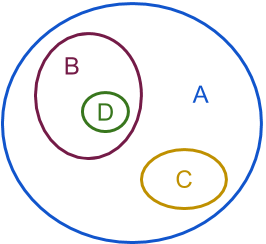
\includegraphics[width=0.27\textwidth]{../figs/nested_spheres.png}
 \caption{2D slice of nested spheres.}
 \label{fig:spheres}
\end{figure}

In the following description of functions, surface meshsets and their corresponding volume meshsets will
together be referred to as objects.  Let us recall that at this point, the volume meshsets do not describe the final volumes
that will be used in transport calculations.  Those will be created during the \texttt{construct\_topology} stage.  
There are a few fundamental assumptions made about the geometry file read in by this tool.
It is assumed that each surface meshset represents a single closed surface, that there are no
overlapping surfaces, and that the only hierarchical relationships that already exist are the parent-child links
within objects.  The surface sense must also be set in each object such that its corresponding volume
meshset is 'inside' the surface meshset.  The \texttt{generate\_hierarchy} class has two main public-facing functions
\texttt{build\_hierarchy} and \texttt{construct\_topology} that can be used in sequence
to prepare a surface mesh geometry for Monte Carlo radiation transport.

\texttt{Build\_hierarchy} tests every object in the geometry and decides where it belongs
in a hierarchical tree.  The hierarchical relationships will be made between volume meshsets.  
The tree is formed by making calls to the DAGMC function \texttt{point\_in\_volume} 
which tests a point on the surface of each volume coming into the tree against the volumes already in the tree.  It will determine if
the point tested is inside or outside of the volume.  Looking again at figure~\ref{fig:spheres}, let us assume that
object A is the first to be tested. The tree is initially empty so volume meshset A is automatically placed at the top.  Assume object C
is tested next.  The point on its surface is found to be inside of volume A, so it becomes a child of A.  Object D is next 
and found to also be inside volume A, but neither inside or outside of volume C.  Volume D becomes another child of A.
Last, object B is tested.  It is found to be inside of A, outside of B, and beside C.  Therefore, volume B becomes a
child of volume A, and a parent of volume D.  Because a volume can only have one parent, the parent-child linkage
between volume A and volume D is broken.  The constructed tree is shown in figure \ref{fig:tree} below.

\begin{figure}[ht] % replace 't' with 'b' to force it to be on the bottom
  \centering
  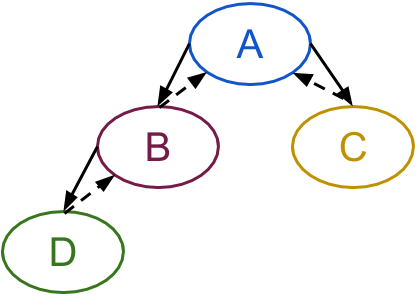
\includegraphics[width=0.3\textwidth]{../figs/tree.png}
  \caption{Hierarchical tree built from nested spheres geometry.  Arrows represent parent-child links.}
  \label{fig:tree}
\end{figure}

After the hierarchical structure has been established, DAGMC-appropriate volumes are created by \texttt{construct\_topology}.
This is accomplished by setting the surface sense and creating parent-child links between the 
surface meshsets.  Each surface has two volumes associated with it, one inside and one outside.  As mentioned earlier,
the surface sense for the 'inside' volume is already set.  This function completes the surface sense data by
setting the 'outside' volume to the volume directly above it in the tree.  Looking at figure \ref{fig:tree},
the 'inside' volume for surface B is set volume B and the 'outside' volume is now set to volume A, 
the parent of volume B.  Because surface A is the outermost surface, 
the 'inside' volume sense is set to volume A but the 'outside' volume sense will be empty.  
Surfaces that have and empty outside volume sense lie in the implicit compliment.

In order to test that the correct hierarchy and topology were being generated by these tools, 
a test problem of nested cubes very similar to the spheres depicted in figure \ref{fig:spheres} was created.
Each cube was represented by a single surface and volume meshset and all other assumptions of a 
pre-\texttt{generate\_hierarchy} geometry were upheld.  In order to test the robustness of the tools,
every permutation of the cube ordering was tested to see if the same hierarchical relationships were
established each time.  For each permutation, \texttt{build\_hierarchy} was called and then
\texttt{construct\_topolgy}.
A \texttt{check\_tree} function was used to ensure that the tree was built during each permutation
matched the reference tree.  

%%%%%%%%%%%%%%%%%%%%%%%%%%%%%%%%%%%%%%%%%%%%%%%%%%%%%%%%%%%%%%%%%%%%%%%%%%%%%%%%
\subsection{Demonstration: Surface Mesh Human Phantom}
In order to demonstrate a real-world use case, we will show how these tools were used to prepare
a polygon surface mesh human phantom for an MCNP5 calculation.  The human phantom was
developed by a group of researchers at the Hanyang University and provided in the OBJ file format.
The OBJ file contained all of the vertex coordinates and connectivity data grouped by object.
The objects in this case are parts of the body.
\texttt{ReadOBJ} was used to read in the file and \texttt{generate\_hierarchy} to instate the correct 
hierarchical relationships and topology.  The \texttt{UW2} process was used to assign materials to
the resulting volumes.  For proof of concept, a DAG-MCNP calculation using a 30 KeV photon
source in the chest was performed.  

Figure~\ref{fig:mcnp} Figure of photon flux in phantom generated by DAG-MCNP
\begin{figure}[ht] % replace 't' with 'b' to force it to be on the bottom
  \centering
  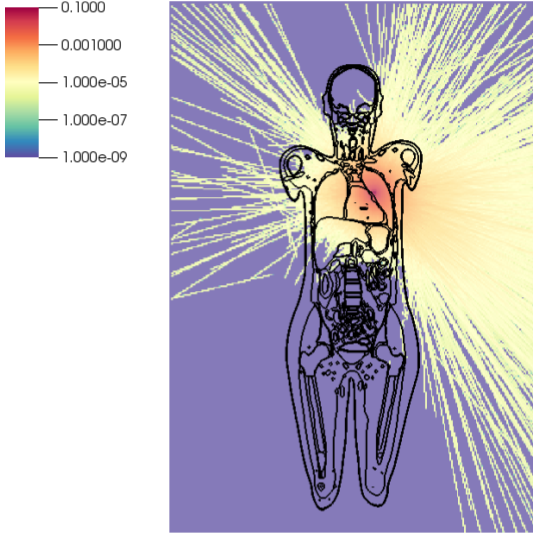
\includegraphics[width=0.5\textwidth]{../figs/30KeV_Psource.png}
  \caption{Photon flux from DAG-MCNP calculation. 30 KeV photon source in chest. }
  \label{fig:mcnp}
\end{figure}

%Figure~\ref{fig:phan_mats} Figure of phantom with materials labeled
%Figure~\ref{fig:fluka} Figure of photon flux in phantom generated by FluDAG 
%Figure~\ref{fig:geant} Figure of photon flux in phantom generated by DAG-Geant

%%%%%%%%%%%%%%%%%%%%%%%%%%%%%%%%%%%%%%%%%%%%%%%%%%%%%%%%%%%%%%%%%%%%%%%%%%%%%%%%
\section{Conclusions and Future Work}

The \texttt{UW2} was developed with the goal of simulating the same Monte Carlo problem with several
physics codes so in the near future, we will run this exact geometry in a FluDAG and DAG-Geant calculation.

%%%%%%%%%%%%%%%%%%%%%%%%%%%%%%%%%%%%%%%%%%%%%%%%%%%%%%%%%%%%%%%%%%%%%%%%%%%%%%%%
\section{Acknowledgments}

%%%%%%%%%%%%%%%%%%%%%%%%%%%%%%%%%%%%%%%%%%%%%%%%%%%%%%%%%%%%%%%%%%%%%%%%%%%%%%%%
\bibliographystyle{ans}
\bibliography{bibliography}
\end{document}

